% ----------------------------------------------------------
\section{Análise dos dados de Monóxido de Carbono}
% ----------------------------------------------------------

\begin{figure}[h]
    \centering
    \caption{Série temporal do sensor CO-B4}
    \begin{subfigure}{0.495\textwidth}
        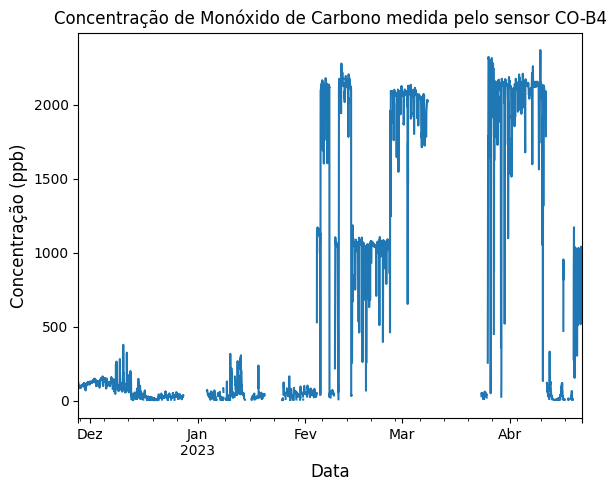
\includegraphics[width=\textwidth]{chapters/3-ANÁLISE DOS DADOS/Figuras/raw-co-b4.png}
        \caption{Série temporal do sensor depois de remover valores fora de intervalo}
        \label{fig:data-co-raw}
    \end{subfigure}
    \hfill
    \begin{subfigure}{0.495\textwidth}
        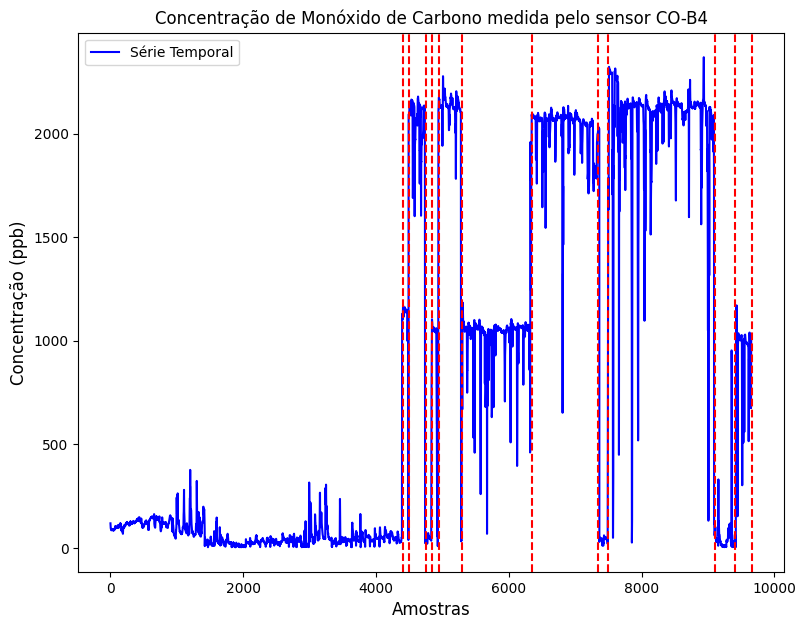
\includegraphics[width=\textwidth]{chapters/3-ANÁLISE DOS DADOS/Figuras/rebase-co-b4.png}
        \caption{Pontos de alteração da linha base detectados pelo algoritmo \acrshort{pelt}}
        \label{fig:data-rebase-co}
    \end{subfigure}
    \hfill
    \label{fig:data-co-raw-and-pelt}
\end{figure}

A metodologia de pre-processamento dos dados descrita acima foi aplicada as leituras obtidas pelo sensor de \acrshort{co}. A Figura \ref{fig:data-co-raw} mostra a série temporal do sensor depois de removidos os valores fora de intervalo. Observa-se que a partir do mês de fevereiro ocorreram seguidas alterações de linha base, detectadas pelo algoritmo \acrshort{pelt}, conforme se ilustra na Figura \ref{fig:data-rebase-co}. No histograma das leituras do sensor em questão (Figura \ref{fig:data-co-raw-hist}) observa-se que as mudanças de linha base alteraram também a distribuição dos dados nesse período. Dado que as mudanças de linha base se mantiveram de forma continuada a partir desse mês, para o restante das análises apenas foram consideradas as leituras anteriores à primeira alteração da linha base do sensor. A Figura \ref{fig:data-co-preproc-hist} mostra o histograma dos dados das leituras prévias às alterações de linha base.

\begin{figure}[h]
    \centering
    \caption{Histograma das leituras do sensor CO-B4}
    \begin{subfigure}{0.4\textwidth}
        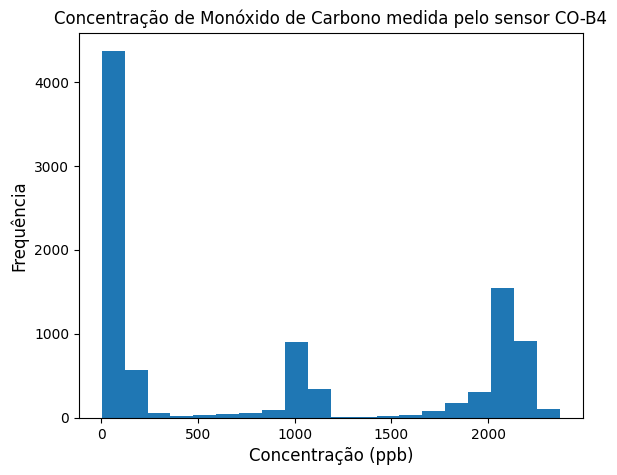
\includegraphics[width=\textwidth]{chapters/3-ANÁLISE DOS DADOS/Figuras/raw-co-b4-hist.png}
        \caption{Histograma prévio à remoção das alterações de linha base}
        \label{fig:data-co-raw-hist}
    \end{subfigure}
    \hfill
    \begin{subfigure}{0.4\textwidth}
        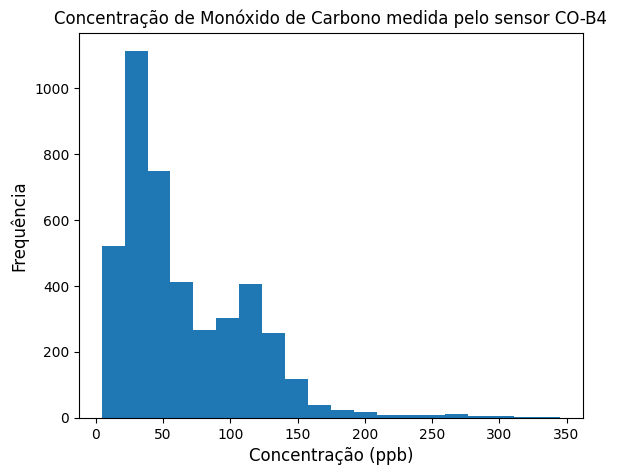
\includegraphics[width=\textwidth]{chapters/3-ANÁLISE DOS DADOS/Figuras/preproc-hist-co-b4.png}
        \caption{Histograma após à remoção das alterações de linha base}
        \label{fig:data-co-preproc-hist}
    \end{subfigure}
    \hfill
    \label{fig:data-co-hist}
\end{figure}

Depois de pré-processadas as leituras do sensor obtiveram-se os resultados ilustrados na Figura \ref{fig:data-co-preproc-15}. A Figura mostra a série de dados pré-processados do sensor CO-B4, juntamente com um gráfico de caixas que representa o comportamento diário das leituras agrupadas por hora do dia. Neste último percebe-se um comportamento periódico nos dados, observando-se maiores valores de amplitude e dispersão durante o período diurno. Ao comparar esse comportamento com os valores de referência percebe-se que a componente diária é mais evidente no sensor CO-B4, indicando uma possível relação com a sazonalidade diária da temperatura.

\begin{figure}[h]
    \centering
    \caption{Série temporal do sensor pré-processada (T = 15 mins) e seu comportamento diário}
    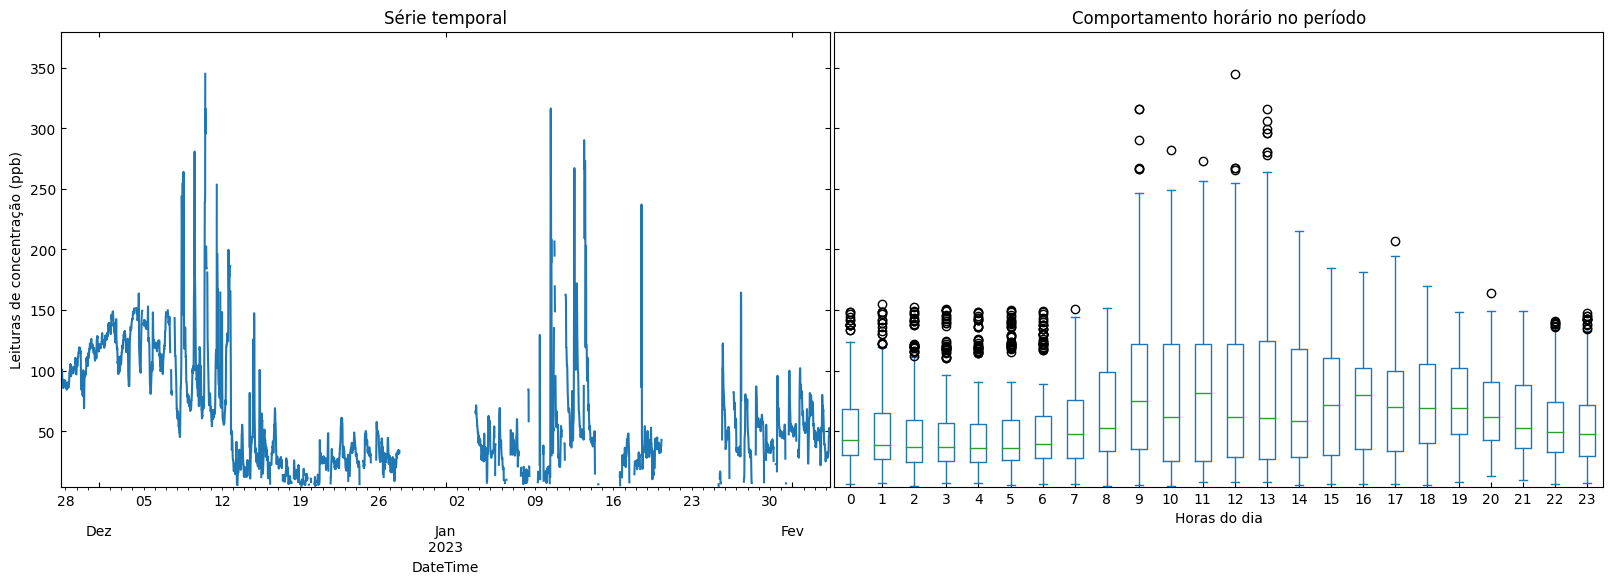
\includegraphics[width=\textwidth]{chapters/3-ANÁLISE DOS DADOS/Figuras/preproc-co-b4.png}
    \label{fig:data-co-preproc-15}
\end{figure}

\begin{figure}[h]
    \centering
    \caption{Série temporal das leituras de concentração de referência (T = 1 H) e seu comportamento diário}
    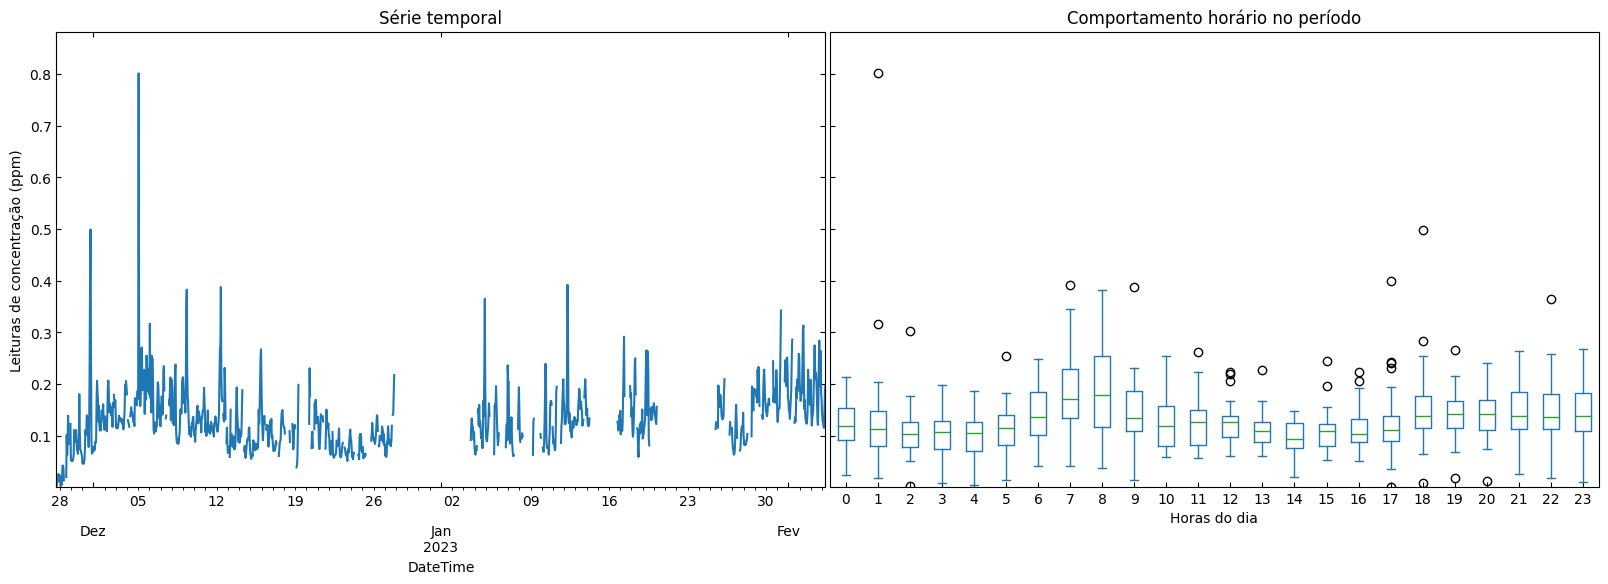
\includegraphics[width=\textwidth]{chapters/3-ANÁLISE DOS DADOS/Figuras/co-reference-series-and-box.png}
    \label{fig:data-co-reference}
\end{figure}

A Figura \ref{fig:data-co-preproc-1HR} mostra a série temporal das leituras do sensor consideradas como válidas, com período de amostragem horário.

\begin{figure}[h]
    \centering
    \caption{Série temporal com T = 1 hr}
    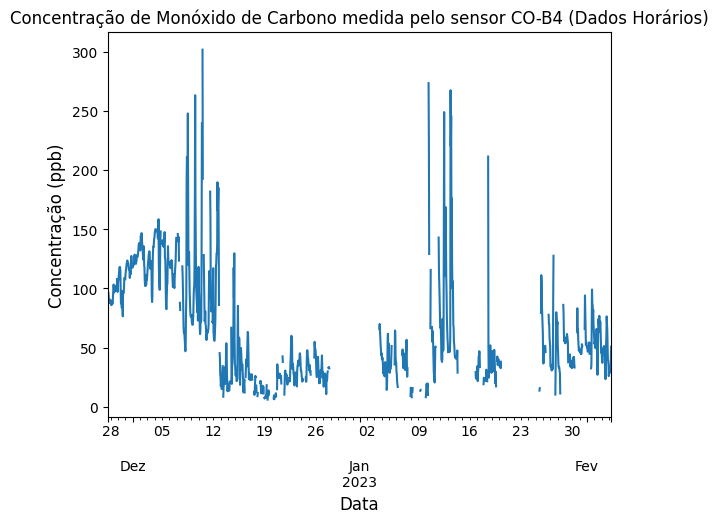
\includegraphics[width=0.5\textwidth]{chapters/3-ANÁLISE DOS DADOS/Figuras/preproc-1HR-co-b4.png}
    \label{fig:data-co-preproc-1HR}
\end{figure}

A Tabela \ref{tab:data-contab-co} mostra a contagem dos dados etiquetados para períodos de 15 minutos e de 1 hora. Observa-se que dos 17647 pontos de dados, que representavam as amostras adquiridas com um período de 15 minutos no intervalo de 20/11/2022 até 23/05/2023, 4270 foram aproveitados como dados válidos, o que representa um 24 \% aproximadamente dos dados originais. Ao re-amostrar esses 4270 pontos em dados horários obtiveram-se 1048 amostras horárias de concentração válidas (aproximadamente 64 \% dos dados) para realizar a calibração.

\begin{table}[h]
    \caption{Contabilização das leituras do sensor CO-B4 por etiquetas}
    \centering
    \begin{tabularx}{0.95\textwidth}[h]{
         >{\raggedright\hsize=.475\hsize\arraybackslash}X
         >{\raggedright\hsize=.20\hsize\arraybackslash}X 
         >{\raggedright\hsize=.5\hsize\arraybackslash}X
        | >{\raggedright\hsize=.50\hsize\arraybackslash}X 
         >{\raggedright\hsize=.20\hsize\arraybackslash}X 
         >{\raggedright\hsize=.5\hsize\arraybackslash}X }
        \multicolumn{3}{c|}{Série temporal T = 15 mins} & \multicolumn{3}{c}{Série temporal T = 1 hr} \\
        \hline
        Etiquetas & No. amostras & \% amostras & Etiquetas & No. amostras & \% amostras \\ [0.5ex]
        \hline
        \textit{MISSING} & 5756 & 32.62 \% & \textit{LOWSAMPLES} & 603 & 36.52 \% \\ [0.5ex]
        
        \textit{LTLL} & 1560 & 8.84 \% & \textit{VALID} & 1048 & 63.48 \% \\ [0.5ex]
        
        \textit{GTUL} & 0.0 & 0.0 \% & & & \\ [0.5ex]
        
        \textit{STABILIZING} & 673 & 3.81 \% & & & \\ [0.5ex]
        
        \textit{BADSPIKE} & 3 & 0.02 \% & & & \\ [0.5ex]
        
        \textit{LTQTLE01} & 63 & 0.36 \% & & & \\ [0.5ex]
        
        \textit{GTQTLE99} & 63 & 0.36 \% & & & \\ [0.5ex]
        
        \textit{REBASE} & 5259 & 29.80 \% & & & \\ [0.5ex]
        
        \textit{VALID} & 4270 & 24.20 \% & & & \\ [0.5ex]
        \hline
        TOTAL & 17647 & & TOTAL & 1651 & \\
    \end{tabularx}
    \label{tab:data-contab-co}
\end{table}

\subsection{Dependência com a temperatura}

Investigou-se a existência de correlação entre as leituras do sensor de \acrshort{co} e as variações de temperatura medida no interior da câmara de medição. Para tal, foram empregados os testes estatísticos de correlação de Spearman e Kendall, por serem métodos não paramétricos que exploram a relação monotônica entre variáveis. Os resultados desses testes revelaram coeficientes de correlação significativos. O coeficiente de Spearman calculado foi de 0.52, com um valor de p inferior a 0.05, indicando uma correlação estatisticamente significativa entre as leituras do sensor e a temperatura. De maneira semelhante, o coeficiente de Kendall foi de 0.38, também com p < 0.05, reforçando a presença de uma associação significativa. Ao avaliar a hipótese nula de ausência de correlação, os resultados forneceram evidências robustas para sua rejeição, sugerindo que há uma correlação entre as leituras do sensor de \acrshort{co} e as variações de temperatura. A Figura \ref{fig:data-temp-co-corr} mostra um gráfico de dispersão entre os dados do sensor e a temperatura, ilustrando os resultados de correlação obtidos. 

\begin{figure}[h]
    \centering
    \caption{Relação dos dados de concentração de \acrshort{co} com a temperatura}
    \begin{subfigure}{0.4\textwidth}
        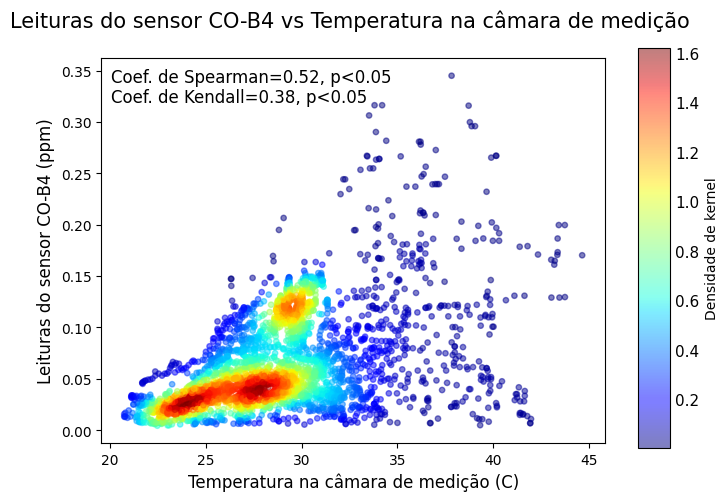
\includegraphics[width=\textwidth]{chapters/3-ANÁLISE DOS DADOS/Figuras/temperature-co-b4.png}
        \caption{Relação entre as leituras do sensor CO-B4 (ppm) e a temperatura (\textdegree C)}
        \label{fig:data-temp-co-corr}
    \end{subfigure}
    \hfill
    \begin{subfigure}{0.4\textwidth}
        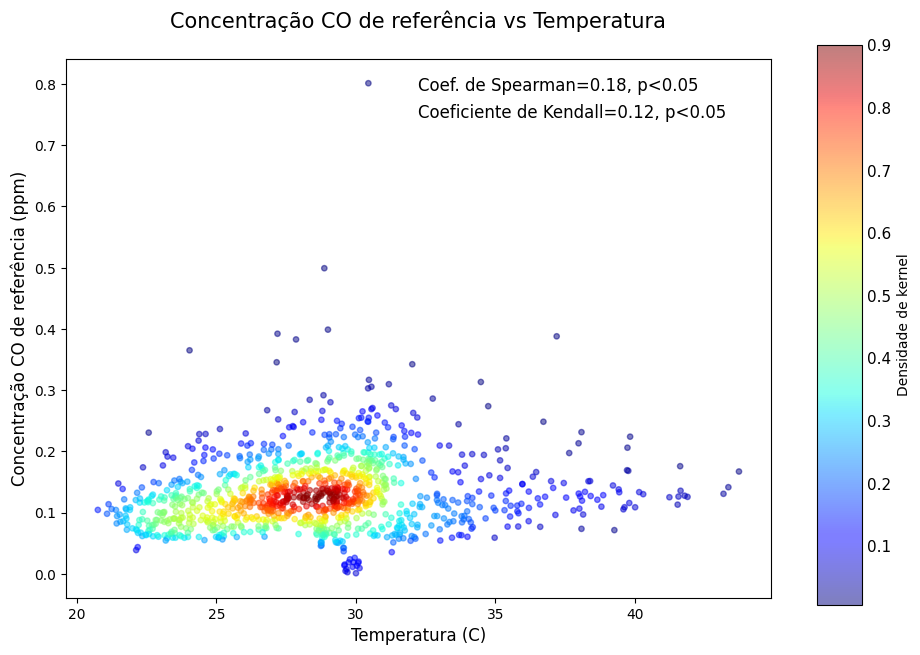
\includegraphics[width=\textwidth]{chapters/3-ANÁLISE DOS DADOS/Figuras/temperature-co-reference.png}
        \caption{Relação entre os valores de concentração de referência (ppm) e a temperatura (\textdegree C)}
        \label{fig:data-temp-co-ref-corr}
    \end{subfigure}
    \hfill
    \label{fig:data-co-temp}
\end{figure}

Os resultados obtidos nos testes estatísticos podem ser corroborados no gráfico de dispersão entre as variáveis. Na Figura \ref{fig:data-temp-co-corr} observam-se dois núcleos principais de dados. O menor deles comporta os valores de concentração entre 0.10 e 0.15 ppm dentro de um intervalo de temperatura de 28 a 30\textdegree C. No segundo núcleo encontram-se valores de concentração entre 0 e 0.06 ppm aproximadamente e de 22 até 30\textdegree C. Neste último grupo de dados é possível apreciar uma clara relação linear entre as leituras do sensor e a temperatura. Ao analisar a relação entre as medições de concentração de referência e a temperatura, também se observa alguma correlação, embora em menor medida, com coeficientes de Spearman e Kendall de 0.18 e 0.12 respectivamente (Figura \ref{fig:data-temp-co-ref-corr}).

\begin{figure}[h]
    \centering
    \caption{Séries temporais e gráficos de dispersão das medições de \acrshort{co}}
    \begin{subfigure}{0.44\textwidth}
        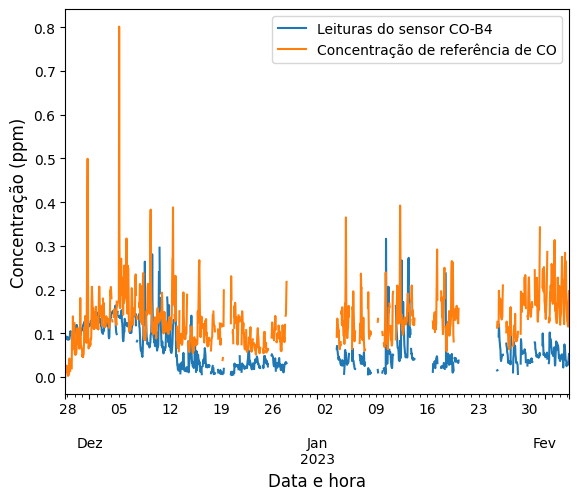
\includegraphics[width=\textwidth]{chapters/3-ANÁLISE DOS DADOS/Figuras/co-b4-reference-time-series.png}
        \caption{Séries temporais das leituras do sensor CO-B4 e a estação de referência}
        \label{fig:data-co-reference-time-series}
    \end{subfigure}
    \hfill
    \begin{subfigure}{0.54\textwidth}
        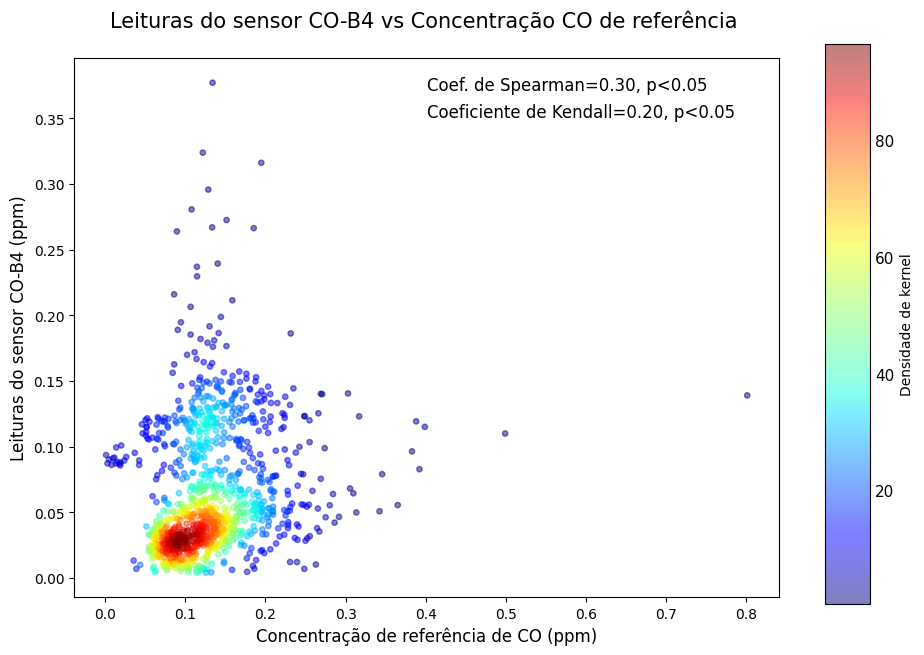
\includegraphics[width=\textwidth]{chapters/3-ANÁLISE DOS DADOS/Figuras/co-b4-reference-correlation.png}
        \caption{Gráfico de dispersão das leituras do sensor CO-B4 e a estação de referência}
        \label{fig:data-co-reference-corr}
    \end{subfigure}
    \fonte{Desenvolvido pelo autor (2023)}
\end{figure}

% ----------------------------------------------------------
\subsection{Comparação das leituras do sensor CO-B4 com as medições de referência}
% ----------------------------------------------------------

Nas Figuras \ref{fig:data-co-reference-time-series} e \ref{fig:data-co-reference-corr} apresentam-se as leituras de \acrshort{co} obtidas pelo sensor CO-B4 de Alphasense e a estação de referência. Observa-se que as leituras do sensor CO-B4 em geral subestimaram os valores de concentração de referência. Os testes de Spearman e Kendall revelaram a existência de correlação entre as medições com o sensor de baixo custo e a referência com coeficientes de 0.3 e 0.2 respectivamente.
